\documentclass[1p]{elsarticle_modified}
%\bibliographystyle{elsarticle-num}

%\usepackage[colorlinks]{hyperref}
%\usepackage{abbrmath_seonhwa} %\Abb, \Ascr, \Acal ,\Abf, \Afrak
\usepackage{amsfonts}
\usepackage{amssymb}
\usepackage{amsmath}
\usepackage{amsthm}
\usepackage{scalefnt}
\usepackage{amsbsy}
\usepackage{kotex}
\usepackage{caption}
\usepackage{subfig}
\usepackage{color}
\usepackage{graphicx}
\usepackage{xcolor} %% white, black, red, green, blue, cyan, magenta, yellow
\usepackage{float}
\usepackage{setspace}
\usepackage{hyperref}

\usepackage{tikz}
\usetikzlibrary{arrows}

\usepackage{multirow}
\usepackage{array} % fixed length table
\usepackage{hhline}

%%%%%%%%%%%%%%%%%%%%%
\makeatletter
\renewcommand*\env@matrix[1][\arraystretch]{%
	\edef\arraystretch{#1}%
	\hskip -\arraycolsep
	\let\@ifnextchar\new@ifnextchar
	\array{*\c@MaxMatrixCols c}}
\makeatother %https://tex.stackexchange.com/questions/14071/how-can-i-increase-the-line-spacing-in-a-matrix
%%%%%%%%%%%%%%%

\usepackage[normalem]{ulem}

\newcommand{\msout}[1]{\ifmmode\text{\sout{\ensuremath{#1}}}\else\sout{#1}\fi}
%SOURCE: \msout is \stkout macro in https://tex.stackexchange.com/questions/20609/strikeout-in-math-mode

\newcommand{\cancel}[1]{
	\ifmmode
	{\color{red}\msout{#1}}
	\else
	{\color{red}\sout{#1}}
	\fi
}

\newcommand{\add}[1]{
	{\color{blue}\uwave{#1}}
}

\newcommand{\replace}[2]{
	\ifmmode
	{\color{red}\msout{#1}}{\color{blue}\uwave{#2}}
	\else
	{\color{red}\sout{#1}}{\color{blue}\uwave{#2}}
	\fi
}

\newcommand{\Sol}{\mathcal{S}} %segment
\newcommand{\D}{D} %diagram
\newcommand{\A}{\mathcal{A}} %arc


%%%%%%%%%%%%%%%%%%%%%%%%%%%%%5 test

\def\sl{\operatorname{\textup{SL}}(2,\Cbb)}
\def\psl{\operatorname{\textup{PSL}}(2,\Cbb)}
\def\quan{\mkern 1mu \triangleright \mkern 1mu}

\theoremstyle{definition}
\newtheorem{thm}{Theorem}[section]
\newtheorem{prop}[thm]{Proposition}
\newtheorem{lem}[thm]{Lemma}
\newtheorem{ques}[thm]{Question}
\newtheorem{cor}[thm]{Corollary}
\newtheorem{defn}[thm]{Definition}
\newtheorem{exam}[thm]{Example}
\newtheorem{rmk}[thm]{Remark}
\newtheorem{alg}[thm]{Algorithm}

\newcommand{\I}{\sqrt{-1}}
\begin{document}

%\begin{frontmatter}
%
%\title{Boundary parabolic representations of knots up to 8 crossings}
%
%%% Group authors per affiliation:
%\author{Yunhi Cho} 
%\address{Department of Mathematics, University of Seoul, Seoul, Korea}
%\ead{yhcho@uos.ac.kr}
%
%
%\author{Seonhwa Kim} %\fnref{s_kim}}
%\address{Center for Geometry and Physics, Institute for Basic Science, Pohang, 37673, Korea}
%\ead{ryeona17@ibs.re.kr}
%
%\author{Hyuk Kim}
%\address{Department of Mathematical Sciences, Seoul National University, Seoul 08826, Korea}
%\ead{hyukkim@snu.ac.kr}
%
%\author{Seokbeom Yoon}
%\address{Department of Mathematical Sciences, Seoul National University, Seoul, 08826,  Korea}
%\ead{sbyoon15@snu.ac.kr}
%
%\begin{abstract}
%We find all boundary parabolic representation of knots up to 8 crossings.
%
%\end{abstract}
%\begin{keyword}
%    \MSC[2010] 57M25 
%\end{keyword}
%
%\end{frontmatter}

%\linenumbers
%\tableofcontents
%
\newcommand\colored[1]{\textcolor{white}{\rule[-0.35ex]{0.8em}{1.4ex}}\kern-0.8em\color{red} #1}%
%\newcommand\colored[1]{\textcolor{white}{ #1}\kern-2.17ex	\textcolor{white}{ #1}\kern-1.81ex	\textcolor{white}{ #1}\kern-2.15ex\color{red}#1	}

{\Large $\underline{12a_{1243}~(K12a_{1243})}$}

\setlength{\tabcolsep}{10pt}
\renewcommand{\arraystretch}{1.6}
\vspace{1cm}\begin{tabular}{m{100pt}>{\centering\arraybackslash}m{274pt}}
\multirow{5}{120pt}{
	\centering
	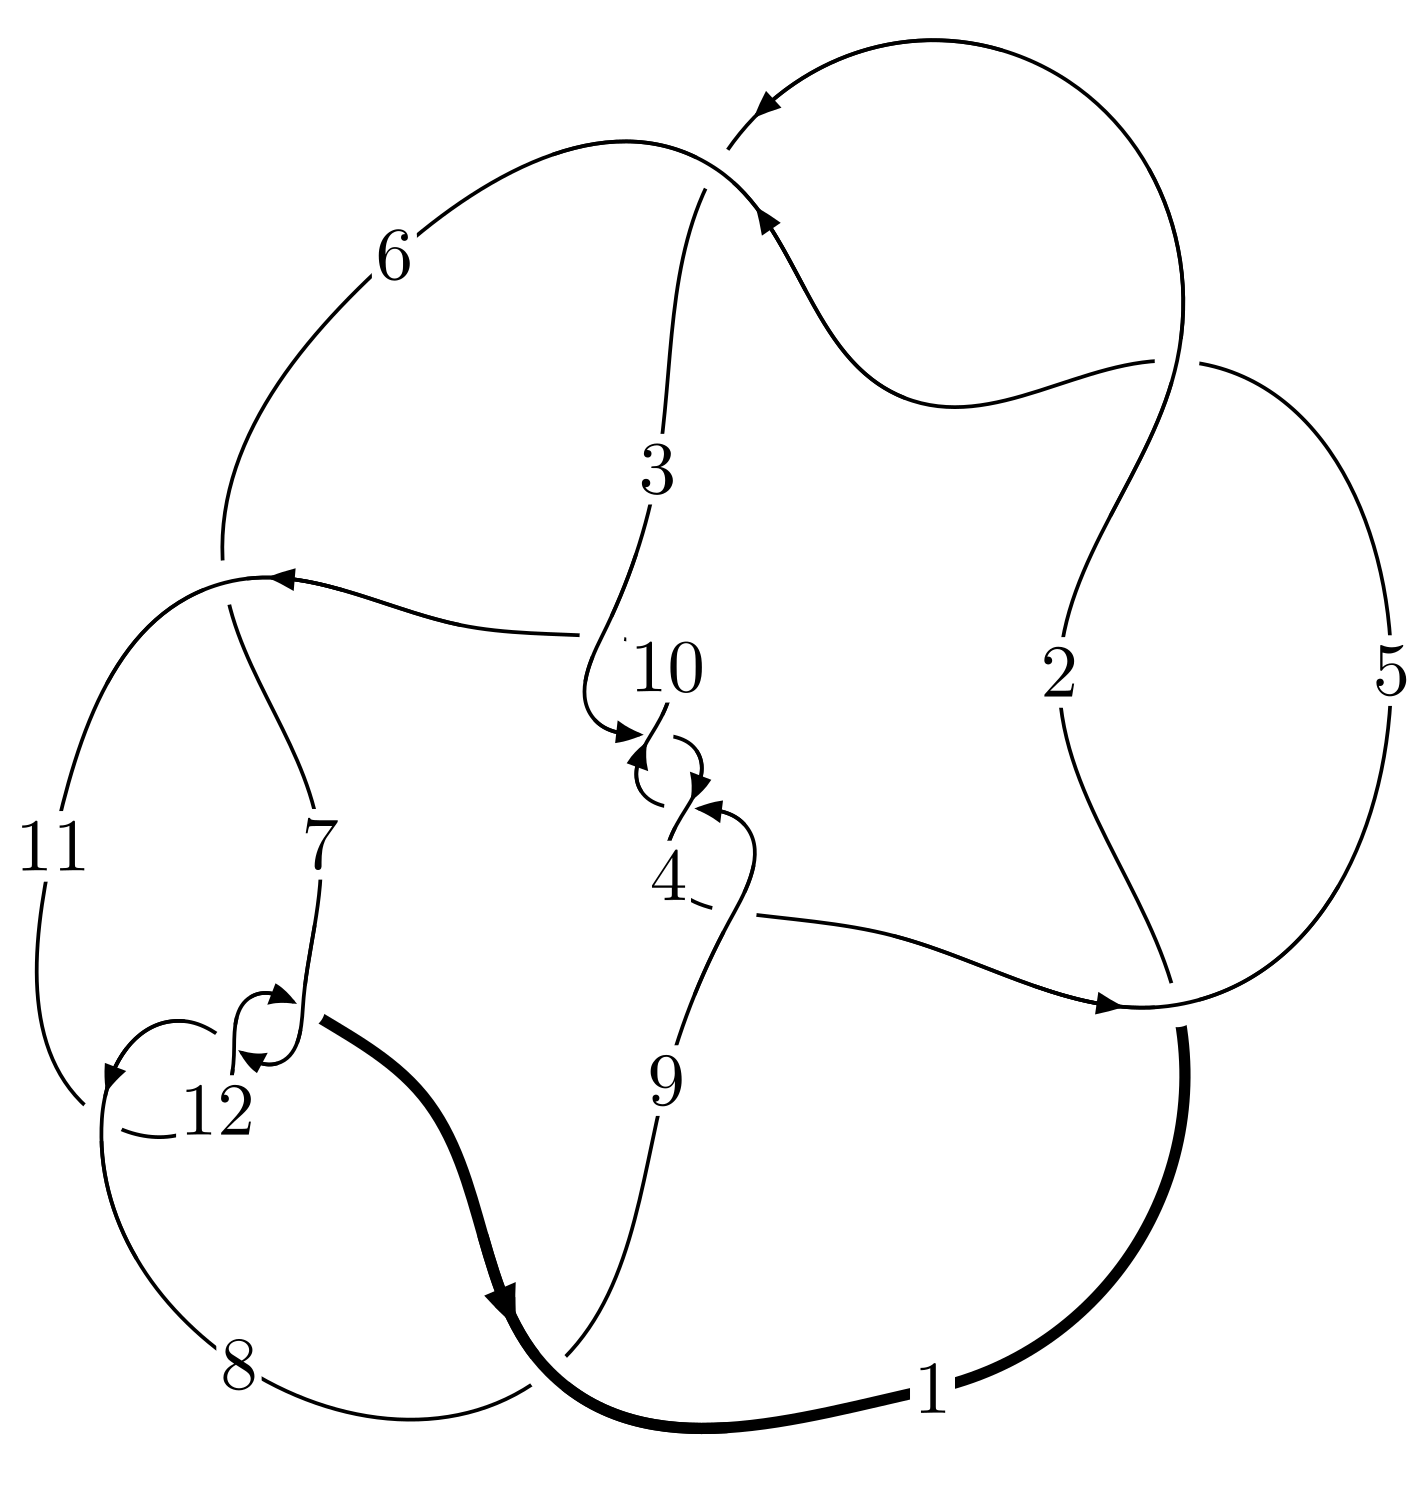
\includegraphics[width=112pt]{../../../GIT/diagram.site/Diagrams/png/2044_12a_1243.png}\\
\ \ \ A knot diagram\footnotemark}&
\allowdisplaybreaks
\textbf{Linearized knot diagam} \\
\cline{2-2}
 &
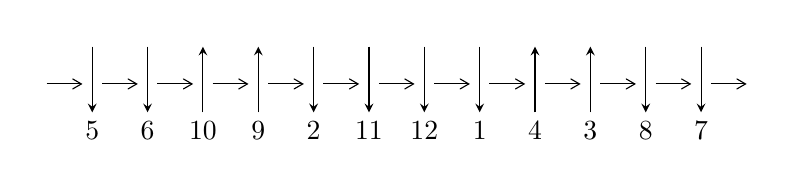
\begin{tikzpicture}[x=20pt, y=17pt]
	% nodes
	\node (C0) at (0, 0) {};
	\node (C1) at (1, 0) {};
	\node (C1U) at (1, +1) {};
	\node (C1D) at (1, -1) {5};

	\node (C2) at (2, 0) {};
	\node (C2U) at (2, +1) {};
	\node (C2D) at (2, -1) {6};

	\node (C3) at (3, 0) {};
	\node (C3U) at (3, +1) {};
	\node (C3D) at (3, -1) {10};

	\node (C4) at (4, 0) {};
	\node (C4U) at (4, +1) {};
	\node (C4D) at (4, -1) {9};

	\node (C5) at (5, 0) {};
	\node (C5U) at (5, +1) {};
	\node (C5D) at (5, -1) {2};

	\node (C6) at (6, 0) {};
	\node (C6U) at (6, +1) {};
	\node (C6D) at (6, -1) {11};

	\node (C7) at (7, 0) {};
	\node (C7U) at (7, +1) {};
	\node (C7D) at (7, -1) {12};

	\node (C8) at (8, 0) {};
	\node (C8U) at (8, +1) {};
	\node (C8D) at (8, -1) {1};

	\node (C9) at (9, 0) {};
	\node (C9U) at (9, +1) {};
	\node (C9D) at (9, -1) {4};

	\node (C10) at (10, 0) {};
	\node (C10U) at (10, +1) {};
	\node (C10D) at (10, -1) {3};

	\node (C11) at (11, 0) {};
	\node (C11U) at (11, +1) {};
	\node (C11D) at (11, -1) {8};

	\node (C12) at (12, 0) {};
	\node (C12U) at (12, +1) {};
	\node (C12D) at (12, -1) {7};
	\node (C13) at (13, 0) {};

	% arrows
	\draw[->,>={angle 60}]
	(C0) edge (C1) (C1) edge (C2) (C2) edge (C3) (C3) edge (C4) (C4) edge (C5) (C5) edge (C6) (C6) edge (C7) (C7) edge (C8) (C8) edge (C9) (C9) edge (C10) (C10) edge (C11) (C11) edge (C12) (C12) edge (C13) ;	\draw[->,>=stealth]
	(C1U) edge (C1D) (C2U) edge (C2D) (C3D) edge (C3U) (C4D) edge (C4U) (C5U) edge (C5D) (C6U) edge (C6D) (C7U) edge (C7D) (C8U) edge (C8D) (C9D) edge (C9U) (C10D) edge (C10U) (C11U) edge (C11D) (C12U) edge (C12D) ;
	\end{tikzpicture} \\
\hhline{~~} \\& 
\textbf{Solving Sequence} \\ \cline{2-2} 
 &
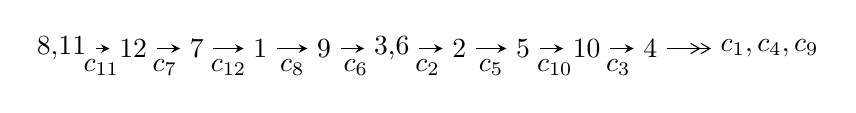
\begin{tikzpicture}[x=23pt, y=7pt]
	% node
	\node (A0) at (-1/8, 0) {8,11};
	\node (A1) at (1, 0) {12};
	\node (A2) at (2, 0) {7};
	\node (A3) at (3, 0) {1};
	\node (A4) at (4, 0) {9};
	\node (A5) at (81/16, 0) {3,6};
	\node (A6) at (49/8, 0) {2};
	\node (A7) at (57/8, 0) {5};
	\node (A8) at (65/8, 0) {10};
	\node (A9) at (73/8, 0) {4};
	\node (C1) at (1/2, -1) {$c_{11}$};
	\node (C2) at (3/2, -1) {$c_{7}$};
	\node (C3) at (5/2, -1) {$c_{12}$};
	\node (C4) at (7/2, -1) {$c_{8}$};
	\node (C5) at (9/2, -1) {$c_{6}$};
	\node (C6) at (45/8, -1) {$c_{2}$};
	\node (C7) at (53/8, -1) {$c_{5}$};
	\node (C8) at (61/8, -1) {$c_{10}$};
	\node (C9) at (69/8, -1) {$c_{3}$};
	\node (A10) at (11, 0) {$c_{1},c_{4},c_{9}$};

	% edge
	\draw[->,>=stealth]	
	(A0) edge (A1) (A1) edge (A2) (A2) edge (A3) (A3) edge (A4) (A4) edge (A5) (A5) edge (A6) (A6) edge (A7) (A7) edge (A8) (A8) edge (A9) ;
	\draw[->>,>={angle 60}]	
	(A9) edge (A10);
\end{tikzpicture} \\ 

\end{tabular} \\

\footnotetext{
The image of knot diagram is generated by the software ``\textbf{Draw programme}" developed by Andrew Bartholomew(\url{http://www.layer8.co.uk/maths/draw/index.htm\#Running-draw}), where we modified some parts for our purpose(\url{https://github.com/CATsTAILs/LinksPainter}).
}\phantom \\ \newline 
\centering \textbf{Ideals for irreducible components\footnotemark of $X_{\text{par}}$} 
 
\begin{align*}
I^u_{1}&=\langle 
5.47710\times10^{15} u^{50}+1.14235\times10^{16} u^{49}+\cdots+3.64380\times10^{16} b-9.84918\times10^{15},\\
\phantom{I^u_{1}}&\phantom{= \langle  }1.63458\times10^{16} u^{50}+1.13811\times10^{16} u^{49}+\cdots+1.09314\times10^{17} a-5.47544\times10^{16},\;u^{51}+2 u^{50}+\cdots-3 u-3\rangle \\
I^u_{2}&=\langle 
- a u- u^2+b+u-1,\;2 u^2 a+a^2+5 u^2+2 a-3 u+8,\;u^3- u^2+2 u-1\rangle \\
I^u_{3}&=\langle 
b,\;u^2+a+1,\;u^3+u^2+2 u+1\rangle \\
\\
\end{align*}
\raggedright * 3 irreducible components of $\dim_{\mathbb{C}}=0$, with total 60 representations.\\
\footnotetext{All coefficients of polynomials are rational numbers. But the coefficients are sometimes approximated in decimal forms when there is not enough margin.}
\newpage
\renewcommand{\arraystretch}{1}
\centering \section*{I. $I^u_{1}= \langle 5.48\times10^{15} u^{50}+1.14\times10^{16} u^{49}+\cdots+3.64\times10^{16} b-9.85\times10^{15},\;1.63\times10^{16} u^{50}+1.14\times10^{16} u^{49}+\cdots+1.09\times10^{17} a-5.48\times10^{16},\;u^{51}+2 u^{50}+\cdots-3 u-3 \rangle$}
\flushleft \textbf{(i) Arc colorings}\\
\begin{tabular}{m{7pt} m{180pt} m{7pt} m{180pt} }
\flushright $a_{8}=$&$\begin{pmatrix}0\\u\end{pmatrix}$ \\
\flushright $a_{11}=$&$\begin{pmatrix}1\\0\end{pmatrix}$ \\
\flushright $a_{12}=$&$\begin{pmatrix}1\\u^2\end{pmatrix}$ \\
\flushright $a_{7}=$&$\begin{pmatrix}u\\u^3+u\end{pmatrix}$ \\
\flushright $a_{1}=$&$\begin{pmatrix}u^2+1\\u^4+2 u^2\end{pmatrix}$ \\
\flushright $a_{9}=$&$\begin{pmatrix}- u^5-2 u^3- u\\- u^7-3 u^5-2 u^3+u\end{pmatrix}$ \\
\flushright $a_{3}=$&$\begin{pmatrix}-0.149530 u^{50}-0.104114 u^{49}+\cdots+4.89363 u+0.500892\\-0.150313 u^{50}-0.313505 u^{49}+\cdots+0.630080 u+0.270300\end{pmatrix}$ \\
\flushright $a_{6}=$&$\begin{pmatrix}u^3+2 u\\u^3+u\end{pmatrix}$ \\
\flushright $a_{2}=$&$\begin{pmatrix}-0.00864236 u^{50}-0.150838 u^{49}+\cdots+4.04860 u+0.105532\\-0.210594 u^{50}-0.927821 u^{49}+\cdots+0.757201 u+0.320503\end{pmatrix}$ \\
\flushright $a_{5}=$&$\begin{pmatrix}-0.106834 u^{50}-0.00307520 u^{49}+\cdots+3.67017 u-0.436697\\0.133553 u^{50}-0.167686 u^{49}+\cdots-0.0796052 u+0.0259271\end{pmatrix}$ \\
\flushright $a_{10}=$&$\begin{pmatrix}0.440680 u^{50}+0.784124 u^{49}+\cdots-2.10894 u+0.0232897\\-0.114496 u^{50}-0.354107 u^{49}+\cdots+1.06838 u+0.0329283\end{pmatrix}$ \\
\flushright $a_{4}=$&$\begin{pmatrix}-0.0918724 u^{50}+0.0332380 u^{49}+\cdots+3.96964 u-0.414486\\0.0811430 u^{50}-0.353168 u^{49}+\cdots+0.231766 u+0.517111\end{pmatrix}$\\&\end{tabular}
\flushleft \textbf{(ii) Obstruction class $= -1$}\\~\\
\flushleft \textbf{(iii) Cusp Shapes $= \frac{7943644690210290}{18218984011570829} u^{50}-\frac{5242160220330023}{18218984011570829} u^{49}+\cdots-\frac{74345173899570890}{18218984011570829} u-\frac{57601482949200522}{18218984011570829}$}\\~\\
\newpage\renewcommand{\arraystretch}{1}
\flushleft \textbf{(iv) u-Polynomials at the component}\newline \\
\begin{tabular}{m{50pt}|m{274pt}}
Crossings & \hspace{64pt}u-Polynomials at each crossing \\
\hline $$\begin{aligned}c_{1},c_{2},c_{5}\end{aligned}$$&$\begin{aligned}
&u^{51}+4 u^{50}+\cdots+44 u-17
\end{aligned}$\\
\hline $$\begin{aligned}c_{3},c_{4},c_{9}\\c_{10}\end{aligned}$$&$\begin{aligned}
&u^{51}+u^{50}+\cdots-124 u^3-8
\end{aligned}$\\
\hline $$\begin{aligned}c_{6},c_{8}\end{aligned}$$&$\begin{aligned}
&u^{51}-2 u^{50}+\cdots-231 u-87
\end{aligned}$\\
\hline $$\begin{aligned}c_{7},c_{11},c_{12}\end{aligned}$$&$\begin{aligned}
&u^{51}+2 u^{50}+\cdots-3 u-3
\end{aligned}$\\
\hline
\end{tabular}\\~\\
\newpage\renewcommand{\arraystretch}{1}
\flushleft \textbf{(v) Riley Polynomials at the component}\newline \\
\begin{tabular}{m{50pt}|m{274pt}}
Crossings & \hspace{64pt}Riley Polynomials at each crossing \\
\hline $$\begin{aligned}c_{1},c_{2},c_{5}\end{aligned}$$&$\begin{aligned}
&y^{51}-56 y^{50}+\cdots+3092 y-289
\end{aligned}$\\
\hline $$\begin{aligned}c_{3},c_{4},c_{9}\\c_{10}\end{aligned}$$&$\begin{aligned}
&y^{51}+65 y^{50}+\cdots+4352 y^2-64
\end{aligned}$\\
\hline $$\begin{aligned}c_{6},c_{8}\end{aligned}$$&$\begin{aligned}
&y^{51}-46 y^{50}+\cdots-73311 y-7569
\end{aligned}$\\
\hline $$\begin{aligned}c_{7},c_{11},c_{12}\end{aligned}$$&$\begin{aligned}
&y^{51}+42 y^{50}+\cdots+57 y-9
\end{aligned}$\\
\hline
\end{tabular}\\~\\
\newpage\flushleft \textbf{(vi) Complex Volumes and Cusp Shapes}
$$\begin{array}{c|c|c}  
\text{Solutions to }I^u_{1}& \I (\text{vol} + \sqrt{-1}CS) & \text{Cusp shape}\\
 \hline 
\begin{aligned}
u &= -0.907928 + 0.131274 I \\
a &= -0.85159 + 2.57553 I \\
b &= \phantom{-}0.17354 + 1.71169 I\end{aligned}
 & \phantom{-}18.9001 + 8.0570 I & -13.49826 - 3.74079 I \\ \hline\begin{aligned}
u &= -0.907928 - 0.131274 I \\
a &= -0.85159 - 2.57553 I \\
b &= \phantom{-}0.17354 - 1.71169 I\end{aligned}
 & \phantom{-}18.9001 - 8.0570 I & -13.49826 + 3.74079 I \\ \hline\begin{aligned}
u &= \phantom{-}0.049806 + 1.119400 I \\
a &= -1.65276 - 0.63158 I \\
b &= \phantom{-}0.14103 - 1.43819 I\end{aligned}
 & -4.53961 - 0.47932 I & -9.08978 - 0.54111 I \\ \hline\begin{aligned}
u &= \phantom{-}0.049806 - 1.119400 I \\
a &= -1.65276 + 0.63158 I \\
b &= \phantom{-}0.14103 + 1.43819 I\end{aligned}
 & -4.53961 + 0.47932 I & -9.08978 + 0.54111 I \\ \hline\begin{aligned}
u &= \phantom{-}0.870747 + 0.070256 I \\
a &= -0.10989 - 1.48062 I \\
b &= \phantom{-}0.608525 - 0.958375 I\end{aligned}
 & -11.35660 - 4.92570 I & -12.66557 + 4.02206 I \\ \hline\begin{aligned}
u &= \phantom{-}0.870747 - 0.070256 I \\
a &= -0.10989 + 1.48062 I \\
b &= \phantom{-}0.608525 + 0.958375 I\end{aligned}
 & -11.35660 + 4.92570 I & -12.66557 - 4.02206 I \\ \hline\begin{aligned}
u &= -0.866790 + 0.044839 I \\
a &= \phantom{-}0.44024 - 3.22463 I \\
b &= -0.05531 - 1.67384 I\end{aligned}
 & -13.05010 + 3.20345 I & -12.09771 - 2.59432 I \\ \hline\begin{aligned}
u &= -0.866790 - 0.044839 I \\
a &= \phantom{-}0.44024 + 3.22463 I \\
b &= -0.05531 + 1.67384 I\end{aligned}
 & -13.05010 - 3.20345 I & -12.09771 + 2.59432 I \\ \hline\begin{aligned}
u &= -0.853858\phantom{ +0.000000I} \\
a &= \phantom{-}0.332469\phantom{ +0.000000I} \\
b &= \phantom{-}0.869508\phantom{ +0.000000I}\end{aligned}
 & -8.45310\phantom{ +0.000000I} & -10.4770\phantom{ +0.000000I} \\ \hline\begin{aligned}
u &= \phantom{-}0.645538 + 0.554017 I \\
a &= \phantom{-}1.09788 + 1.43143 I \\
b &= -0.02763 + 1.69086 I\end{aligned}
 & -14.2712 - 2.2782 I & -11.91209 + 2.93097 I\\
 \hline 
 \end{array}$$\newpage$$\begin{array}{c|c|c}  
\text{Solutions to }I^u_{1}& \I (\text{vol} + \sqrt{-1}CS) & \text{Cusp shape}\\
 \hline 
\begin{aligned}
u &= \phantom{-}0.645538 - 0.554017 I \\
a &= \phantom{-}1.09788 - 1.43143 I \\
b &= -0.02763 - 1.69086 I\end{aligned}
 & -14.2712 + 2.2782 I & -11.91209 - 2.93097 I \\ \hline\begin{aligned}
u &= \phantom{-}0.098307 + 1.231160 I \\
a &= -1.087560 + 0.607902 I \\
b &= \phantom{-}0.422786 + 0.380273 I\end{aligned}
 & \phantom{-}1.39334 - 1.58061 I & -4.00000 + 0. I\phantom{ +0.000000I} \\ \hline\begin{aligned}
u &= \phantom{-}0.098307 - 1.231160 I \\
a &= -1.087560 - 0.607902 I \\
b &= \phantom{-}0.422786 - 0.380273 I\end{aligned}
 & \phantom{-}1.39334 + 1.58061 I & -4.00000 + 0. I\phantom{ +0.000000I} \\ \hline\begin{aligned}
u &= \phantom{-}0.761889 + 0.030162 I \\
a &= \phantom{-}0.14348 + 1.84705 I \\
b &= -0.227333 + 0.836438 I\end{aligned}
 & -4.19077 - 2.14878 I & -11.40445 + 4.59039 I \\ \hline\begin{aligned}
u &= \phantom{-}0.761889 - 0.030162 I \\
a &= \phantom{-}0.14348 - 1.84705 I \\
b &= -0.227333 - 0.836438 I\end{aligned}
 & -4.19077 + 2.14878 I & -11.40445 - 4.59039 I \\ \hline\begin{aligned}
u &= -0.488015 + 1.149550 I \\
a &= -0.480142 + 1.284100 I \\
b &= -0.14196 + 1.72564 I\end{aligned}
 & -17.4585 - 3.1002 I & \phantom{-0.000000 } 0 \\ \hline\begin{aligned}
u &= -0.488015 - 1.149550 I \\
a &= -0.480142 - 1.284100 I \\
b &= -0.14196 - 1.72564 I\end{aligned}
 & -17.4585 + 3.1002 I & \phantom{-0.000000 } 0 \\ \hline\begin{aligned}
u &= \phantom{-}0.303333 + 1.240150 I \\
a &= \phantom{-}0.481754 + 0.904540 I \\
b &= \phantom{-}0.082101 + 0.850538 I\end{aligned}
 & -0.47130 - 1.69507 I & \phantom{-0.000000 } 0 \\ \hline\begin{aligned}
u &= \phantom{-}0.303333 - 1.240150 I \\
a &= \phantom{-}0.481754 - 0.904540 I \\
b &= \phantom{-}0.082101 - 0.850538 I\end{aligned}
 & -0.47130 + 1.69507 I & \phantom{-0.000000 } 0 \\ \hline\begin{aligned}
u &= \phantom{-}0.418137 + 1.207070 I \\
a &= -0.181479 - 0.248186 I \\
b &= -0.556081 - 1.021520 I\end{aligned}
 & -7.85706 + 0.30900 I & \phantom{-0.000000 } 0\\
 \hline 
 \end{array}$$\newpage$$\begin{array}{c|c|c}  
\text{Solutions to }I^u_{1}& \I (\text{vol} + \sqrt{-1}CS) & \text{Cusp shape}\\
 \hline 
\begin{aligned}
u &= \phantom{-}0.418137 - 1.207070 I \\
a &= -0.181479 + 0.248186 I \\
b &= -0.556081 + 1.021520 I\end{aligned}
 & -7.85706 - 0.30900 I & \phantom{-0.000000 } 0 \\ \hline\begin{aligned}
u &= -0.052017 + 1.294910 I \\
a &= \phantom{-}0.953642 - 0.051833 I \\
b &= -0.447473 - 0.419214 I\end{aligned}
 & \phantom{-}4.49060 + 1.57458 I & \phantom{-0.000000 } 0 \\ \hline\begin{aligned}
u &= -0.052017 - 1.294910 I \\
a &= \phantom{-}0.953642 + 0.051833 I \\
b &= -0.447473 + 0.419214 I\end{aligned}
 & \phantom{-}4.49060 - 1.57458 I & \phantom{-0.000000 } 0 \\ \hline\begin{aligned}
u &= -0.410167 + 1.234410 I \\
a &= \phantom{-}0.96089 - 1.81167 I \\
b &= \phantom{-}0.01537 - 1.67225 I\end{aligned}
 & -9.37724 + 1.37166 I & \phantom{-0.000000 } 0 \\ \hline\begin{aligned}
u &= -0.410167 - 1.234410 I \\
a &= \phantom{-}0.96089 + 1.81167 I \\
b &= \phantom{-}0.01537 + 1.67225 I\end{aligned}
 & -9.37724 - 1.37166 I & \phantom{-0.000000 } 0 \\ \hline\begin{aligned}
u &= -0.259573 + 1.277840 I \\
a &= -0.313273 + 0.355431 I \\
b &= \phantom{-}0.450243 - 0.039258 I\end{aligned}
 & \phantom{-}2.27192 + 3.32252 I & \phantom{-0.000000 } 0 \\ \hline\begin{aligned}
u &= -0.259573 - 1.277840 I \\
a &= -0.313273 - 0.355431 I \\
b &= \phantom{-}0.450243 + 0.039258 I\end{aligned}
 & \phantom{-}2.27192 - 3.32252 I & \phantom{-0.000000 } 0 \\ \hline\begin{aligned}
u &= \phantom{-}0.332771 + 1.284440 I \\
a &= -1.05807 - 1.05291 I \\
b &= \phantom{-}0.338435 - 0.828395 I\end{aligned}
 & -0.09882 - 6.10554 I & \phantom{-0.000000 } 0 \\ \hline\begin{aligned}
u &= \phantom{-}0.332771 - 1.284440 I \\
a &= -1.05807 + 1.05291 I \\
b &= \phantom{-}0.338435 + 0.828395 I\end{aligned}
 & -0.09882 + 6.10554 I & \phantom{-0.000000 } 0 \\ \hline\begin{aligned}
u &= -0.393305 + 1.273120 I \\
a &= \phantom{-}0.441102 - 0.573712 I \\
b &= -0.865536 + 0.073675 I\end{aligned}
 & -4.49930 + 4.47398 I & \phantom{-0.000000 } 0\\
 \hline 
 \end{array}$$\newpage$$\begin{array}{c|c|c}  
\text{Solutions to }I^u_{1}& \I (\text{vol} + \sqrt{-1}CS) & \text{Cusp shape}\\
 \hline 
\begin{aligned}
u &= -0.393305 - 1.273120 I \\
a &= \phantom{-}0.441102 + 0.573712 I \\
b &= -0.865536 - 0.073675 I\end{aligned}
 & -4.49930 - 4.47398 I & \phantom{-0.000000 } 0 \\ \hline\begin{aligned}
u &= -0.660643\phantom{ +0.000000I} \\
a &= -0.232662\phantom{ +0.000000I} \\
b &= -0.401553\phantom{ +0.000000I}\end{aligned}
 & -1.71027\phantom{ +0.000000I} & -3.43300\phantom{ +0.000000I} \\ \hline\begin{aligned}
u &= \phantom{-}0.148769 + 1.331880 I \\
a &= \phantom{-}1.213820 - 0.003770 I \\
b &= -0.05720 + 1.47291 I\end{aligned}
 & -1.60931 - 3.17982 I & \phantom{-0.000000 } 0 \\ \hline\begin{aligned}
u &= \phantom{-}0.148769 - 1.331880 I \\
a &= \phantom{-}1.213820 + 0.003770 I \\
b &= -0.05720 - 1.47291 I\end{aligned}
 & -1.60931 + 3.17982 I & \phantom{-0.000000 } 0 \\ \hline\begin{aligned}
u &= -0.487213 + 0.407368 I \\
a &= \phantom{-}0.952102 - 0.113234 I \\
b &= -0.144630 - 0.903505 I\end{aligned}
 & -5.05412 + 1.66912 I & -10.97373 - 4.62737 I \\ \hline\begin{aligned}
u &= -0.487213 - 0.407368 I \\
a &= \phantom{-}0.952102 + 0.113234 I \\
b &= -0.144630 + 0.903505 I\end{aligned}
 & -5.05412 - 1.66912 I & -10.97373 + 4.62737 I \\ \hline\begin{aligned}
u &= -0.397349 + 1.308030 I \\
a &= -1.65562 + 1.61052 I \\
b &= \phantom{-}0.08962 + 1.66718 I\end{aligned}
 & -8.82655 + 7.73768 I & \phantom{-0.000000 } 0 \\ \hline\begin{aligned}
u &= -0.397349 - 1.308030 I \\
a &= -1.65562 - 1.61052 I \\
b &= \phantom{-}0.08962 - 1.66718 I\end{aligned}
 & -8.82655 - 7.73768 I & \phantom{-0.000000 } 0 \\ \hline\begin{aligned}
u &= \phantom{-}0.396413 + 1.325070 I \\
a &= \phantom{-}1.20491 + 0.91251 I \\
b &= -0.640552 + 0.900828 I\end{aligned}
 & -6.99006 - 9.47255 I & \phantom{-0.000000 } 0 \\ \hline\begin{aligned}
u &= \phantom{-}0.396413 - 1.325070 I \\
a &= \phantom{-}1.20491 - 0.91251 I \\
b &= -0.640552 - 0.900828 I\end{aligned}
 & -6.99006 + 9.47255 I & \phantom{-0.000000 } 0\\
 \hline 
 \end{array}$$\newpage$$\begin{array}{c|c|c}  
\text{Solutions to }I^u_{1}& \I (\text{vol} + \sqrt{-1}CS) & \text{Cusp shape}\\
 \hline 
\begin{aligned}
u &= -0.153785 + 1.383640 I \\
a &= -0.828540 - 0.587282 I \\
b &= \phantom{-}0.236607 + 0.683213 I\end{aligned}
 & \phantom{-}0.58476 + 3.87146 I & \phantom{-0.000000 } 0 \\ \hline\begin{aligned}
u &= -0.153785 - 1.383640 I \\
a &= -0.828540 + 0.587282 I \\
b &= \phantom{-}0.236607 - 0.683213 I\end{aligned}
 & \phantom{-}0.58476 - 3.87146 I & \phantom{-0.000000 } 0 \\ \hline\begin{aligned}
u &= -0.40573 + 1.36865 I \\
a &= \phantom{-}1.84188 - 1.07241 I \\
b &= -0.19235 - 1.69170 I\end{aligned}
 & -15.8596 + 12.7667 I & \phantom{-0.000000 } 0 \\ \hline\begin{aligned}
u &= -0.40573 - 1.36865 I \\
a &= \phantom{-}1.84188 + 1.07241 I \\
b &= -0.19235 + 1.69170 I\end{aligned}
 & -15.8596 - 12.7667 I & \phantom{-0.000000 } 0 \\ \hline\begin{aligned}
u &= \phantom{-}0.15668 + 1.46609 I \\
a &= -0.952170 + 0.297878 I \\
b &= \phantom{-}0.06047 - 1.64270 I\end{aligned}
 & -7.63888 - 4.94907 I & \phantom{-0.000000 } 0 \\ \hline\begin{aligned}
u &= \phantom{-}0.15668 - 1.46609 I \\
a &= -0.952170 - 0.297878 I \\
b &= \phantom{-}0.06047 + 1.64270 I\end{aligned}
 & -7.63888 + 4.94907 I & \phantom{-0.000000 } 0 \\ \hline\begin{aligned}
u &= \phantom{-}0.424316 + 0.265115 I \\
a &= -1.41012 - 2.43053 I \\
b &= -0.00144 - 1.49759 I\end{aligned}
 & -6.57052 - 1.14577 I & -8.04300 + 6.02810 I \\ \hline\begin{aligned}
u &= \phantom{-}0.424316 - 0.265115 I \\
a &= -1.41012 + 2.43053 I \\
b &= -0.00144 + 1.49759 I\end{aligned}
 & -6.57052 + 1.14577 I & -8.04300 - 6.02810 I \\ \hline\begin{aligned}
u &= \phantom{-}0.351513\phantom{ +0.000000I} \\
a &= \phantom{-}2.15459\phantom{ +0.000000I} \\
b &= -0.342179\phantom{ +0.000000I}\end{aligned}
 & -2.23327\phantom{ +0.000000I} & \phantom{-}1.33350\phantom{ +0.000000I} \\ \hline\begin{aligned}
u &= -0.203339 + 0.264461 I \\
a &= -0.777669 + 0.662838 I \\
b &= \phantom{-}0.175873 + 0.407856 I\end{aligned}
 & -0.158036 + 0.749712 I & -4.84555 - 9.27744 I\\
 \hline 
 \end{array}$$\newpage$$\begin{array}{c|c|c}  
\text{Solutions to }I^u_{1}& \I (\text{vol} + \sqrt{-1}CS) & \text{Cusp shape}\\
 \hline 
\begin{aligned}
u &= -0.203339 - 0.264461 I \\
a &= -0.777669 - 0.662838 I \\
b &= \phantom{-}0.175873 - 0.407856 I\end{aligned}
 & -0.158036 - 0.749712 I & -4.84555 + 9.27744 I\\
 \hline 
 \end{array}$$\newpage\newpage\renewcommand{\arraystretch}{1}
\centering \section*{II. $I^u_{2}= \langle - a u- u^2+b+u-1,\;2 u^2 a+a^2+5 u^2+2 a-3 u+8,\;u^3- u^2+2 u-1 \rangle$}
\flushleft \textbf{(i) Arc colorings}\\
\begin{tabular}{m{7pt} m{180pt} m{7pt} m{180pt} }
\flushright $a_{8}=$&$\begin{pmatrix}0\\u\end{pmatrix}$ \\
\flushright $a_{11}=$&$\begin{pmatrix}1\\0\end{pmatrix}$ \\
\flushright $a_{12}=$&$\begin{pmatrix}1\\u^2\end{pmatrix}$ \\
\flushright $a_{7}=$&$\begin{pmatrix}u\\u^2- u+1\end{pmatrix}$ \\
\flushright $a_{1}=$&$\begin{pmatrix}u^2+1\\u^2- u+1\end{pmatrix}$ \\
\flushright $a_{9}=$&$\begin{pmatrix}-1\\0\end{pmatrix}$ \\
\flushright $a_{3}=$&$\begin{pmatrix}a\\a u+u^2- u+1\end{pmatrix}$ \\
\flushright $a_{6}=$&$\begin{pmatrix}u^2+1\\u^2- u+1\end{pmatrix}$ \\
\flushright $a_{2}=$&$\begin{pmatrix}u^2+a+1\\a u+2 u^2-2 u+2\end{pmatrix}$ \\
\flushright $a_{5}=$&$\begin{pmatrix}- a\\- a u- u^2+u-1\end{pmatrix}$ \\
\flushright $a_{10}=$&$\begin{pmatrix}- u^2 a+a u-2 u^2- a+2 u-4\\-2\end{pmatrix}$ \\
\flushright $a_{4}=$&$\begin{pmatrix}a u+u^2- a- u+1\\- a u- u^2+u-1\end{pmatrix}$\\&\end{tabular}
\flushleft \textbf{(ii) Obstruction class $= 1$}\\~\\
\flushleft \textbf{(iii) Cusp Shapes $= -4 u^2+4 u-16$}\\~\\
\newpage\renewcommand{\arraystretch}{1}
\flushleft \textbf{(iv) u-Polynomials at the component}\newline \\
\begin{tabular}{m{50pt}|m{274pt}}
Crossings & \hspace{64pt}u-Polynomials at each crossing \\
\hline $$\begin{aligned}c_{1},c_{2}\end{aligned}$$&$\begin{aligned}
&(u+1)^6
\end{aligned}$\\
\hline $$\begin{aligned}c_{3},c_{4},c_{9}\\c_{10}\end{aligned}$$&$\begin{aligned}
&(u^2+2)^3
\end{aligned}$\\
\hline $$\begin{aligned}c_{5}\end{aligned}$$&$\begin{aligned}
&(u-1)^6
\end{aligned}$\\
\hline $$\begin{aligned}c_{6},c_{8}\end{aligned}$$&$\begin{aligned}
&(u^3- u^2+1)^2
\end{aligned}$\\
\hline $$\begin{aligned}c_{7}\end{aligned}$$&$\begin{aligned}
&(u^3+u^2+2 u+1)^2
\end{aligned}$\\
\hline $$\begin{aligned}c_{11},c_{12}\end{aligned}$$&$\begin{aligned}
&(u^3- u^2+2 u-1)^2
\end{aligned}$\\
\hline
\end{tabular}\\~\\
\newpage\renewcommand{\arraystretch}{1}
\flushleft \textbf{(v) Riley Polynomials at the component}\newline \\
\begin{tabular}{m{50pt}|m{274pt}}
Crossings & \hspace{64pt}Riley Polynomials at each crossing \\
\hline $$\begin{aligned}c_{1},c_{2},c_{5}\end{aligned}$$&$\begin{aligned}
&(y-1)^6
\end{aligned}$\\
\hline $$\begin{aligned}c_{3},c_{4},c_{9}\\c_{10}\end{aligned}$$&$\begin{aligned}
&(y+2)^6
\end{aligned}$\\
\hline $$\begin{aligned}c_{6},c_{8}\end{aligned}$$&$\begin{aligned}
&(y^3- y^2+2 y-1)^2
\end{aligned}$\\
\hline $$\begin{aligned}c_{7},c_{11},c_{12}\end{aligned}$$&$\begin{aligned}
&(y^3+3 y^2+2 y-1)^2
\end{aligned}$\\
\hline
\end{tabular}\\~\\
\newpage\flushleft \textbf{(vi) Complex Volumes and Cusp Shapes}
$$\begin{array}{c|c|c}  
\text{Solutions to }I^u_{2}& \I (\text{vol} + \sqrt{-1}CS) & \text{Cusp shape}\\
 \hline 
\begin{aligned}
u &= \phantom{-}0.215080 + 1.307140 I \\
a &= -0.391035 - 0.735607 I \\
b &= \phantom{-0.000000 } -1.414210 I\end{aligned}
 & -3.55561 - 2.82812 I & -8.49024 + 2.97945 I \\ \hline\begin{aligned}
u &= \phantom{-}0.215080 + 1.307140 I \\
a &= \phantom{-}1.71575 - 0.38895 I \\
b &= \phantom{-0.000000 -}1.414210 I\end{aligned}
 & -3.55561 - 2.82812 I & -8.49024 + 2.97945 I \\ \hline\begin{aligned}
u &= \phantom{-}0.215080 - 1.307140 I \\
a &= -0.391035 + 0.735607 I \\
b &= \phantom{-0.000000 -}1.414210 I\end{aligned}
 & -3.55561 + 2.82812 I & -8.49024 - 2.97945 I \\ \hline\begin{aligned}
u &= \phantom{-}0.215080 - 1.307140 I \\
a &= \phantom{-}1.71575 + 0.38895 I \\
b &= \phantom{-0.000000 } -1.414210 I\end{aligned}
 & -3.55561 + 2.82812 I & -8.49024 - 2.97945 I \\ \hline\begin{aligned}
u &= \phantom{-}0.569840\phantom{ +0.000000I} \\
a &= -1.32472 + 2.48177 I \\
b &= \phantom{-0.000000 -}1.414210 I\end{aligned}
 & -7.69319\phantom{ +0.000000I} & -15.0200\phantom{ +0.000000I} \\ \hline\begin{aligned}
u &= \phantom{-}0.569840\phantom{ +0.000000I} \\
a &= -1.32472 - 2.48177 I \\
b &= \phantom{-0.000000 } -1.414210 I\end{aligned}
 & -7.69319\phantom{ +0.000000I} & -15.0200\phantom{ +0.000000I}\\
 \hline 
 \end{array}$$\newpage\newpage\renewcommand{\arraystretch}{1}
\centering \section*{III. $I^u_{3}= \langle b,\;u^2+a+1,\;u^3+u^2+2 u+1 \rangle$}
\flushleft \textbf{(i) Arc colorings}\\
\begin{tabular}{m{7pt} m{180pt} m{7pt} m{180pt} }
\flushright $a_{8}=$&$\begin{pmatrix}0\\u\end{pmatrix}$ \\
\flushright $a_{11}=$&$\begin{pmatrix}1\\0\end{pmatrix}$ \\
\flushright $a_{12}=$&$\begin{pmatrix}1\\u^2\end{pmatrix}$ \\
\flushright $a_{7}=$&$\begin{pmatrix}u\\- u^2- u-1\end{pmatrix}$ \\
\flushright $a_{1}=$&$\begin{pmatrix}u^2+1\\u^2+u+1\end{pmatrix}$ \\
\flushright $a_{9}=$&$\begin{pmatrix}1\\0\end{pmatrix}$ \\
\flushright $a_{3}=$&$\begin{pmatrix}- u^2-1\\0\end{pmatrix}$ \\
\flushright $a_{6}=$&$\begin{pmatrix}- u^2-1\\- u^2- u-1\end{pmatrix}$ \\
\flushright $a_{2}=$&$\begin{pmatrix}0\\u^2+u+1\end{pmatrix}$ \\
\flushright $a_{5}=$&$\begin{pmatrix}- u^2-1\\0\end{pmatrix}$ \\
\flushright $a_{10}=$&$\begin{pmatrix}1\\0\end{pmatrix}$ \\
\flushright $a_{4}=$&$\begin{pmatrix}- u^2-1\\0\end{pmatrix}$\\&\end{tabular}
\flushleft \textbf{(ii) Obstruction class $= 1$}\\~\\
\flushleft \textbf{(iii) Cusp Shapes $= -6 u^2-4 u-16$}\\~\\
\newpage\renewcommand{\arraystretch}{1}
\flushleft \textbf{(iv) u-Polynomials at the component}\newline \\
\begin{tabular}{m{50pt}|m{274pt}}
Crossings & \hspace{64pt}u-Polynomials at each crossing \\
\hline $$\begin{aligned}c_{1},c_{2}\end{aligned}$$&$\begin{aligned}
&(u-1)^3
\end{aligned}$\\
\hline $$\begin{aligned}c_{3},c_{4},c_{9}\\c_{10}\end{aligned}$$&$\begin{aligned}
&u^3
\end{aligned}$\\
\hline $$\begin{aligned}c_{5}\end{aligned}$$&$\begin{aligned}
&(u+1)^3
\end{aligned}$\\
\hline $$\begin{aligned}c_{6},c_{8}\end{aligned}$$&$\begin{aligned}
&u^3+u^2-1
\end{aligned}$\\
\hline $$\begin{aligned}c_{7}\end{aligned}$$&$\begin{aligned}
&u^3- u^2+2 u-1
\end{aligned}$\\
\hline $$\begin{aligned}c_{11},c_{12}\end{aligned}$$&$\begin{aligned}
&u^3+u^2+2 u+1
\end{aligned}$\\
\hline
\end{tabular}\\~\\
\newpage\renewcommand{\arraystretch}{1}
\flushleft \textbf{(v) Riley Polynomials at the component}\newline \\
\begin{tabular}{m{50pt}|m{274pt}}
Crossings & \hspace{64pt}Riley Polynomials at each crossing \\
\hline $$\begin{aligned}c_{1},c_{2},c_{5}\end{aligned}$$&$\begin{aligned}
&(y-1)^3
\end{aligned}$\\
\hline $$\begin{aligned}c_{3},c_{4},c_{9}\\c_{10}\end{aligned}$$&$\begin{aligned}
&y^3
\end{aligned}$\\
\hline $$\begin{aligned}c_{6},c_{8}\end{aligned}$$&$\begin{aligned}
&y^3- y^2+2 y-1
\end{aligned}$\\
\hline $$\begin{aligned}c_{7},c_{11},c_{12}\end{aligned}$$&$\begin{aligned}
&y^3+3 y^2+2 y-1
\end{aligned}$\\
\hline
\end{tabular}\\~\\
\newpage\flushleft \textbf{(vi) Complex Volumes and Cusp Shapes}
$$\begin{array}{c|c|c}  
\text{Solutions to }I^u_{3}& \I (\text{vol} + \sqrt{-1}CS) & \text{Cusp shape}\\
 \hline 
\begin{aligned}
u &= -0.215080 + 1.307140 I \\
a &= \phantom{-}0.662359 + 0.562280 I \\
b &= \phantom{-0.000000 } 0\end{aligned}
 & \phantom{-}1.37919 + 2.82812 I & -5.16553 - 1.85489 I \\ \hline\begin{aligned}
u &= -0.215080 - 1.307140 I \\
a &= \phantom{-}0.662359 - 0.562280 I \\
b &= \phantom{-0.000000 } 0\end{aligned}
 & \phantom{-}1.37919 - 2.82812 I & -5.16553 + 1.85489 I \\ \hline\begin{aligned}
u &= -0.569840\phantom{ +0.000000I} \\
a &= -1.32472\phantom{ +0.000000I} \\
b &= \phantom{-0.000000 } 0\end{aligned}
 & -2.75839\phantom{ +0.000000I} & -15.6690\phantom{ +0.000000I}\\
 \hline 
 \end{array}$$\newpage
\newpage\renewcommand{\arraystretch}{1}
\centering \section*{ IV. u-Polynomials}
\begin{tabular}{m{50pt}|m{274pt}}
Crossings & \hspace{64pt}u-Polynomials at each crossing \\
\hline $$\begin{aligned}c_{1},c_{2}\end{aligned}$$&$\begin{aligned}
&((u-1)^3)(u+1)^6(u^{51}+4 u^{50}+\cdots+44 u-17)
\end{aligned}$\\
\hline $$\begin{aligned}c_{3},c_{4},c_{9}\\c_{10}\end{aligned}$$&$\begin{aligned}
&u^3(u^2+2)^3(u^{51}+u^{50}+\cdots-124 u^3-8)
\end{aligned}$\\
\hline $$\begin{aligned}c_{5}\end{aligned}$$&$\begin{aligned}
&((u-1)^6)(u+1)^3(u^{51}+4 u^{50}+\cdots+44 u-17)
\end{aligned}$\\
\hline $$\begin{aligned}c_{6},c_{8}\end{aligned}$$&$\begin{aligned}
&((u^3- u^2+1)^2)(u^3+u^2-1)(u^{51}-2 u^{50}+\cdots-231 u-87)
\end{aligned}$\\
\hline $$\begin{aligned}c_{7}\end{aligned}$$&$\begin{aligned}
&(u^3- u^2+2 u-1)(u^3+u^2+2 u+1)^2(u^{51}+2 u^{50}+\cdots-3 u-3)
\end{aligned}$\\
\hline $$\begin{aligned}c_{11},c_{12}\end{aligned}$$&$\begin{aligned}
&((u^3- u^2+2 u-1)^2)(u^3+u^2+2 u+1)(u^{51}+2 u^{50}+\cdots-3 u-3)
\end{aligned}$\\
\hline
\end{tabular}\newpage\renewcommand{\arraystretch}{1}
\centering \section*{ V. Riley Polynomials}
\begin{tabular}{m{50pt}|m{274pt}}
Crossings & \hspace{64pt}Riley Polynomials at each crossing \\
\hline $$\begin{aligned}c_{1},c_{2},c_{5}\end{aligned}$$&$\begin{aligned}
&((y-1)^9)(y^{51}-56 y^{50}+\cdots+3092 y-289)
\end{aligned}$\\
\hline $$\begin{aligned}c_{3},c_{4},c_{9}\\c_{10}\end{aligned}$$&$\begin{aligned}
&y^3(y+2)^6(y^{51}+65 y^{50}+\cdots+4352 y^{2}-64)
\end{aligned}$\\
\hline $$\begin{aligned}c_{6},c_{8}\end{aligned}$$&$\begin{aligned}
&((y^3- y^2+2 y-1)^3)(y^{51}-46 y^{50}+\cdots-73311 y-7569)
\end{aligned}$\\
\hline $$\begin{aligned}c_{7},c_{11},c_{12}\end{aligned}$$&$\begin{aligned}
&((y^3+3 y^2+2 y-1)^3)(y^{51}+42 y^{50}+\cdots+57 y-9)
\end{aligned}$\\
\hline
\end{tabular}
\vskip 2pc
\end{document}